\section{Density-based Methods}

\begin{frame}{Density-based Clustering}
	\begin{itemize}
		\item \textbf{Clustering based on density (local cluster criterion),
			      such as density-connected points.}
		\item \textbf{Major features:}
		      \begin{itemize}
			      \item Discover clusters of arbitrary shape.
			      \item Handle noise.
			      \item One scan.
			      \item Need density parameters as termination condition.
		      \end{itemize}
		\item \textbf{Several interesting studies:}
		      \begin{itemize}
			      \item DBSCAN\footfullcite{ester1996}.
			      \item OPTICS\footfullcite{ankerst1999-2}.
			      \item DENCLUE\footfullcite{hinneburg1998}.
			      \item CLIQUE\footfullcite{agarwal1998}(more grid-based).
		      \end{itemize}
	\end{itemize}
\end{frame}

\begin{frame}{Density-based Clustering: Basic Concepts}
	\begin{itemize}
		\item \textbf{Two parameters:}
		      \begin{itemize}
			      \item \textbf{\color{airforceblue}$\epsilon$}: Maximum radius of a
			            neighborhood.
			            \begin{itemize}
				            \item Defines the neighborhood of a point $p$: $N_{\epsilon}(p)
					                  := \{q \in D \; \vert \; d(p,q) \leq \epsilon\}$.
				            \item Distance function is still needed.
			            \end{itemize}
			      \item \textbf{\color{airforceblue}MinPts}: Minimum number of points
			            in an $\epsilon$-neighborhood of a point $p$.
		      \end{itemize}
		\item \textbf{{\color{airforceblue}Core-point condition:}
		      $|N_{\epsilon}(p)| \geq \text{MinPts}$.}
		      \begin{itemize}
			      \item Only these neighborhoods are considered.
		      \end{itemize}
	\end{itemize}
	\centering
	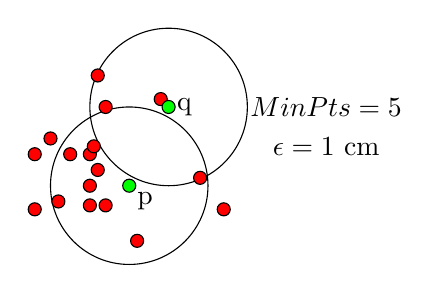
\begin{tikzpicture}
		\draw (0,0) circle (1cm);
		\draw (-0.5,-1) circle (1cm);
		\node[draw, circle, fill=red, scale=0.5] at (-1,-1) {};
		\node[draw, circle, fill=red, scale=0.5] at (-0.8,0) {};
		\node[draw, circle, fill=red, scale=0.5] at (-0.9,0.4) {};
		\node[draw, circle, fill=red, scale=0.5] at (-0.1,0.1) {};
		\node[draw, circle, fill=red, scale=0.5] at (0.4,-0.9) {};
		\node[draw, circle, fill=red, scale=0.5] at (0.7,-1.3) {};
		\node[draw, circle, fill=red, scale=0.5] at (-1.5,-0.4) {};
		\node[draw, circle, fill=red, scale=0.5] at (-1,-0.6) {};
		\node[draw, circle, fill=red, scale=0.5] at (-0.9,-0.8) {};
		\node[draw, circle, fill=red, scale=0.5] at (-0.95,-0.5) {};
		\node[draw, circle, fill=red, scale=0.5] at (-1.25,-0.6) {};
		\node[draw, circle, fill=red, scale=0.5] at (-1.7,-0.6) {};
		\node[draw, circle, fill=red, scale=0.5] at (-1.7,-1.3) {};
		\node[draw, circle, fill=red, scale=0.5] at (-1.4,-1.2) {};
		\node[draw, circle, fill=red, scale=0.5] at (-1,-1.25) {};
		\node[draw, circle, fill=red, scale=0.5] at (-0.8,-1.25) {};
		\node[draw, circle, fill=red, scale=0.5] at (-0.4,-1.7) {};
		\node[draw, circle, fill=green, scale=0.5] at (-0.5,-1) {};
		\node[draw, circle, fill=green, scale=0.5] at (0,0) {};
		\node at (0.2,0) {q};
		\node at (-0.3,-1.2) {p};
		\node at (2,0) {$\text{MinPts} = 5$};
		\node at (2,-0.5) {$\epsilon = 1$ cm};
	\end{tikzpicture}
\end{frame}

\begin{frame}{Directly Density-reachable}
	\begin{itemize}
		\item A point $q$ is said to be directly density-reachable from a point
		      $p$ \\
		      w.r.t. $\epsilon$, MinPts, if $q$ belongs to $N_{\epsilon}(p)$.
	\end{itemize}
	\centering
	\vspace{0.5cm}
	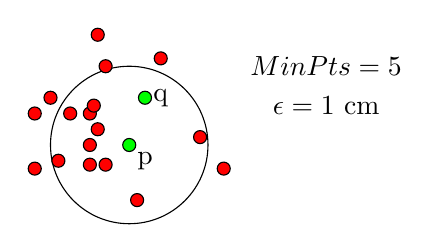
\begin{tikzpicture}
		\draw (-0.5,-1) circle (1cm);
		\node[draw, circle, fill=red, scale=0.5] at (-1,-1) {};
		\node[draw, circle, fill=red, scale=0.5] at (-0.8,0) {};
		\node[draw, circle, fill=red, scale=0.5] at (-0.9,0.4) {};
		\node[draw, circle, fill=red, scale=0.5] at (-0.1,0.1) {};
		\node[draw, circle, fill=red, scale=0.5] at (0.4,-0.9) {};
		\node[draw, circle, fill=red, scale=0.5] at (0.7,-1.3) {};
		\node[draw, circle, fill=red, scale=0.5] at (-1.5,-0.4) {};
		\node[draw, circle, fill=red, scale=0.5] at (-1,-0.6) {};
		\node[draw, circle, fill=red, scale=0.5] at (-0.9,-0.8) {};
		\node[draw, circle, fill=red, scale=0.5] at (-0.95,-0.5) {};
		\node[draw, circle, fill=red, scale=0.5] at (-1.25,-0.6) {};
		\node[draw, circle, fill=red, scale=0.5] at (-1.7,-0.6) {};
		\node[draw, circle, fill=red, scale=0.5] at (-1.7,-1.3) {};
		\node[draw, circle, fill=red, scale=0.5] at (-1.4,-1.2) {};
		\node[draw, circle, fill=red, scale=0.5] at (-1,-1.25) {};
		\node[draw, circle, fill=red, scale=0.5] at (-0.8,-1.25) {};
		\node[draw, circle, fill=red, scale=0.5] at (-0.4,-1.7) {};
		\node[draw, circle, fill=green, scale=0.5] at (-0.5,-1) {};
		\node[draw, circle, fill=green, scale=0.5] at (-0.3,-0.4) {};
		\node at (-0.1,-0.4) {q};
		\node at (-0.3,-1.2) {p};
		\node at (2,0) {$\text{MinPts} = 5$};
		\node at (2,-0.5) {$\epsilon = 1$ cm};
	\end{tikzpicture}
\end{frame}

\begin{frame}{Density-reachable and Density-connected}
	\begin{itemize}
		\item \textbf{\color{airforceblue}Density-reachable:}
		      \begin{itemize}
			      \item A point $q$ is density-reachable from a point $p$ w.r.t.
			            $\epsilon$, MinPts, if there is a \textbf{chain of points} $p_1,
				            \ldots, p_n$, $p_1 = p$, $p_n = q$ such that $p_i+1$ is directly
			            density-reachable from $p_i$.\\[0.2cm]
			            \centering
			            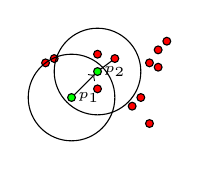
\begin{tikzpicture}[scale=1.1]
				            \node[draw, circle, fill=red, scale=0.3] at (0.3,0.1) {};
				            \node[draw, circle, fill=red, scale=0.3] at (0.3,0.5) {};
				            \node[draw, circle, fill=red, scale=0.3] at (-0.3,0.4) {};
				            \node[draw, circle, fill=red, scale=0.3] at (-0.2,0.45) {};
				            \node[draw, circle, fill=red, scale=0.3] at (0.5,0.45) (p3) {};
				            \node[draw, circle, fill=red, scale=0.3] at (0.8,0) {};
				            \node[draw, circle, fill=red, scale=0.3] at (0.7,-0.1) {};
				            \node[draw, circle, fill=red, scale=0.3] at (0.9,-0.3) {};
				            \node[draw, circle, fill=red, scale=0.3] at (0.9,0.4) {};
				            \node[draw, circle, fill=red, scale=0.3] at (1,0.55) {};
				            \node[draw, circle, fill=red, scale=0.3] at (1,0.35) {};
				            \node[draw, circle, fill=red, scale=0.3] at (1.1,0.65) {};

				            \draw (0,0) circle (0.5cm);
				            \node[draw, circle, fill=green, scale=0.3] at (0,0) (p1) {};
				            \node at (0.2,0) {\tiny$p_1$};
				            \draw (0.3,0.3) circle (0.5cm);
				            \node[draw, circle, fill=green, scale=0.3] at (0.3,0.3) (p2) {};
				            \node at (0.5,0.3) {\tiny$p_2$};
				            \draw[->] (p1)--(p2);
				            \draw (p2)--(p3);
			            \end{tikzpicture}
		      \end{itemize}
		\item \textbf{\color{airforceblue}Density-connected:}
		      \begin{itemize}
			      \item A point $p$ is density-connected to a point $q$ w.r.t.
			            $\epsilon$, MinPts, if there is a point $o$ such that both $p$ and
			            $q$ are density-reachable from $o$. \\[0.2cm]
			            \centering
			            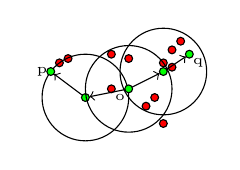
\begin{tikzpicture}[scale=1.1]
				            \node[draw, circle, fill=red, scale=0.3] at (0.3,0.1) {};
				            \node[draw, circle, fill=red, scale=0.3] at (0.3,0.5) {};
				            \node[draw, circle, fill=red, scale=0.3] at (-0.3,0.4) {};
				            \node[draw, circle, fill=red, scale=0.3] at (-0.2,0.45) {};
				            \node[draw, circle, fill=red, scale=0.3] at (0.5,0.45) (p3) {};
				            \node[draw, circle, fill=red, scale=0.3] at (0.8,0) {};
				            \node[draw, circle, fill=red, scale=0.3] at (0.7,-0.1) {};
				            \node[draw, circle, fill=red, scale=0.3] at (0.9,-0.3) {};
				            \node[draw, circle, fill=red, scale=0.3] at (0.9,0.4) {};
				            \node[draw, circle, fill=red, scale=0.3] at (1,0.55) {};
				            \node[draw, circle, fill=red, scale=0.3] at (1,0.35) {};
				            \node[draw, circle, fill=red, scale=0.3] at (1.1,0.65) {};
				            \draw (0,0) circle (0.5cm);
				            \node[draw, circle, fill=green, scale=0.3] at (0,0) (p1) {};
				            \draw (0.5,0.1) circle (0.5cm);
				            \node[draw, circle, fill=green, scale=0.3] at (0.5,0.1) (p2) {};
				            \node at (0.4,0) {\tiny o};
				            \draw (0.9,0.3) circle (0.5cm);
				            \node[draw, circle, fill=green, scale=0.3] at (0.9,0.3) (p3) {};
				            \node[draw, circle, fill=green, scale=0.3] at (-0.4,0.3) (p4)
				            {};
				            \node at (-0.5,0.3) {\tiny p};
				            \node[draw, circle, fill=green, scale=0.3] at (1.2,0.5) (p5) {};
				            \node at (1.3,0.4) {\tiny q};
				            \draw[->] (p2)--(p3);
				            \draw[->] (p2)--(p1);
				            \draw[->] (p3)--(p5);
				            \draw[->] (p1)--(p4);
			            \end{tikzpicture}
		      \end{itemize}
	\end{itemize}
\end{frame}

\begin{frame}{DBSCAN: Density-based Spatial Clustering of Applications with
		Noise}
	\begin{itemize}
		\item \textbf{Relies on a density-based notion of cluster:}
		      \begin{itemize}
			      \item A cluster is defined as a maximal set of density-connected
			            points.
		      \end{itemize}
		\item \textbf{Discovers clusters of arbitrary shape in spatial
			      databases with noise.}
	\end{itemize}
	\centering
	\vspace{0.5cm}
	\scalebox{0.85}{
		\begin{tikzpicture}
			\draw (0,0) rectangle (6,4);
			\node[draw, circle, fill=airforceblue] at (1.6,0.55) {};
			\node[draw, circle, fill=airforceblue] at (1.4,0.85) {};
			\node[draw, circle, fill=airforceblue] at (1.75,0.95) {};
			\node[draw, circle, fill=airforceblue] at (1.25,1.8) (core) {};
			\draw[dashed] (1.25,1.8) circle (0.7cm);

			\node[draw, circle, fill=airforceblue] at (1.25,2.3) {};
			\node[draw, circle, fill=airforceblue] at (0.8,1.75) {};
			\node[draw, circle, fill=airforceblue] at (1.6,1.85) {};
			\node[draw, circle, fill=airforceblue] at (1.1,1.25) {};
			\node[draw, circle, fill=airforceblue] at (1.7,1.5) {};
			\node[draw, circle, fill=airforceblue] at (1.2,3.2) (border) {};
			\node[draw, circle, fill=airforceblue] at (0.8,2.8) {};
			\node[draw, circle, fill=airforceblue] at (1.8,2.8) {};
			\node[draw, circle, fill=airforceblue] at (1.8,3.2) {};

			\node[draw, circle, fill=airforceblue] at (4.3,1.5) {};
			\node[draw, circle, fill=airforceblue] at (4.1,1.2) {};
			\node[draw, circle, fill=airforceblue] at (3.8,1.8) {};
			\node[draw, circle, fill=airforceblue] at (4,2.1) {};
			\node[draw, circle, fill=airforceblue] at (4.1,1.2) {};
			\draw[dashed] (0.8,3.2) circle (0.7cm);
			\node[draw, circle, fill=airforceblue] at (4.8,3.2) (outlier) {};
			\draw[dashed] (4.4,3) circle (0.7cm);
			\node[draw, fill=white] at (6,3.2) (o) {Outlier};
			\node[draw, fill=white] at (-1,1.2) (c) {Core};
			\node[draw, fill=white] at (-1,2.2) (b) {Border};
			\node at (7,2.2) {$\epsilon$ = 1cm};
			\node at (7,1.7) {MinPts = 5};
			\draw (outlier)--(o);
			\draw (core)--(c);
			\draw (border)--(b);
		\end{tikzpicture}
	}
\end{frame}

\begin{frame}{DBSCAN: The Algorithm}
	\begin{itemize}
		\item All objects in database $D$ are marked \texttt{unvisited}.
		\item Randomly select unvisited object $p$ and mark as \texttt{visited}.
		\item If $\epsilon$-neighborhood of $p$ contains less than MinPts
		      objects:
		      \begin{itemize}
			      \item Mark $p$ as noise.
		      \end{itemize}
		\item Otherwise (that is, $p$ is core point):
		      \begin{itemize}
			      \item Create new cluster $C$ for point $p$.
			      \item Add all objects in $\epsilon$-neighborhood of $p$ to
			            candidate set $N$.
			      \item For each $p'$ in $N$ that does not yet belong to a cluster:
			            \begin{itemize}
				            \item Add $p'$ to $C$.
				            \item If $p'$ is \texttt{unvisited}, mark as \texttt{visited}.
				            \item If $p'$ is core point, add all objects in its
				                  $\epsilon$-neighborhood to $N$.
			            \end{itemize}
			      \item Ends when $N$ is empty, that is, $C$ can no longer be
			            expanded.
		      \end{itemize}
		\item Continue the process (randomly select next unvisited object in
		      $D$) until all points have been visited.
	\end{itemize}
\end{frame}

\begin{frame}{DBSCAN: Sensitive to Parameters}
	\centering
	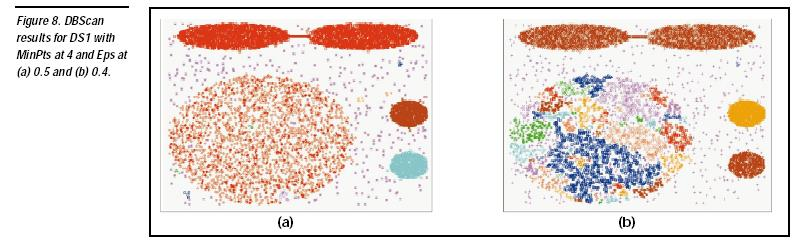
\includegraphics[width=12cm]{img/dbscan.png}\\
	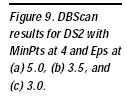
\includegraphics[width=2cm]{img/dbscan3.png}
	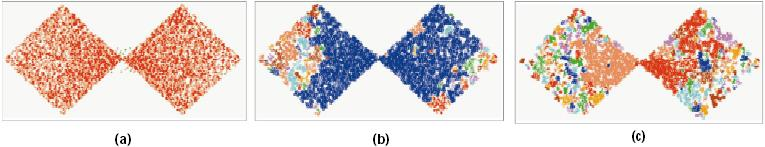
\includegraphics[width=10cm]{img/dbscan2.png}
\end{frame}

\begin{frame}{OPTICS: A Cluster-ordering Method}
	\begin{itemize}
		\item \textbf{OPTICS: Ordering Points To Identify the Clustering
			      Structure.}\footfullcite{ankerst1999-2}
		      \begin{itemize}
			      \item Avoid difficulty of finding the right parameters:
			            \begin{itemize}
				            \item Only MinPts must be given, $\epsilon$ remains open.
			            \end{itemize}
			      \item Produces a special \textbf{order of the database} w.r.t. its
			            density-based clustering structure.
			      \item This cluster-ordering contains info equivalent to the
			            density-based clusterings \\ corresponding to a broad range of
			            parameter settings.
			      \item Good for both automatic and interactive cluster analysis,
			            including finding \\
			            intrinsic clustering structure.
			      \item Can be represented graphically or using visualization
			            techniques.
			      \item Process point in order: Select a point that is
			            density-reachable w.r.t. the lowest $\epsilon$ value, so that
			            clusters with higher density (lower $\epsilon$) will be finished
			            first.
		      \end{itemize}
	\end{itemize}
\end{frame}

\begin{frame}{OPTICS: Some Extension of DBSCAN}
	\begin{columns}
		\begin{column}{0.7\textwidth}
			\vspace{-4cm}
			\begin{itemize}
				\item \textbf{\color{airforceblue}Core distance:}
				      \begin{itemize}
					      \item of a point $p$.
					      \item Min $\epsilon$ s.t. $p$ is core point.
				      \end{itemize}
				\item \textbf{\color{airforceblue}Reachability Distance $r$:}
				      \begin{itemize}
					      \item of a point $p$ from $q$.
					      \item Minimum radius value that makes $p$ \\ directly
					            density-reachable from $q$.
					      \item That is, $r(q,p) := \max\{\text{core-distance}(q),
						            d(q,p)\}$.
				      \end{itemize}
				\item \textbf{Example:}
				      \begin{itemize}
					      \item MinPts $= 5$, core\_distance$(q) = 3cm$.
					      \item $d(q,p_1) = 2.8 cm \implies r(q, p_1) = 3cm$.
					      \item $d(q,p_2) = 4 cm \implies r(q, p_2) = 4 cm$.
				      \end{itemize}
			\end{itemize}
		\end{column}
		\begin{column}{0.3\textwidth}
			\centering
			\vspace{4cm}
			\begin{tikzpicture}
				\draw (0,0) circle (2cm);
				\draw (0,0) circle (1cm);
				\node[draw, circle, fill=airforceblue] at (0,0) (c) {};
				\node[draw, circle, fill=airforceblue] at (-2,0) (p2) {};
				\node[draw, circle, fill=airforceblue] at (-0.1,0.5) (p1) {};
				\node[draw, circle, fill=airforceblue] at (-0.7,0.1) {};
				\node[draw, circle, fill=airforceblue] at (0.8,0.05) {};
				\node[draw, circle, fill=airforceblue] at (0.4,-0.7) {};
				\node[draw, circle, fill=airforceblue] at (0.5,1) {};
				\node at (0.3,0) {$q$};
				\node at (-1.65,-0.2) {$p_2$};
				\node at (-0.4,0.5) {$p_1$};
				\draw (c)--(p2);
				\draw (c)--(p1);
			\end{tikzpicture}
		\end{column}
	\end{columns}
\end{frame}

\begin{frame}{OPTICS: Algorithm}
	\begin{itemize}
		\item \textbf{Maintains a list of {\color{airforceblue}OrderSeeds}:}
		      \begin{itemize}
			      \item Points sorted by \textbf{reachability-distance} from their
			            resp. closest core points.
		      \end{itemize}
		\item \textbf{Begin with arbitrary point from input DB.}
		\item \textbf{For each point $p$ under consideration:}
		      \begin{itemize}
			      \item Retrieve the closest MinPts points of $p$, determine
			            core-distance, set reachability-distance to undefined.
			      \item Write $p$ to output.
			      \item If $p$ is core point, for each point $q$ in the
			            $\epsilon$-neighborhood of $p$:
			            \begin{itemize}
				            \item Update reachability-distance from $p$.
				            \item Insert $q$ into OrderSeeds (if $q$ has not yet been
				                  processed).
			            \end{itemize}
			      \item Move to next object in OrderSeeds list with smallest
			            reachability-distance (or input DB if OrderSeeds is empty).
		      \end{itemize}
		\item \textbf{Continue until input DB fully consumed (and OrderSeeds
			      empty).}
	\end{itemize}
\end{frame}

\begin{frame}{OPTICS: Visualization}
	\centering
	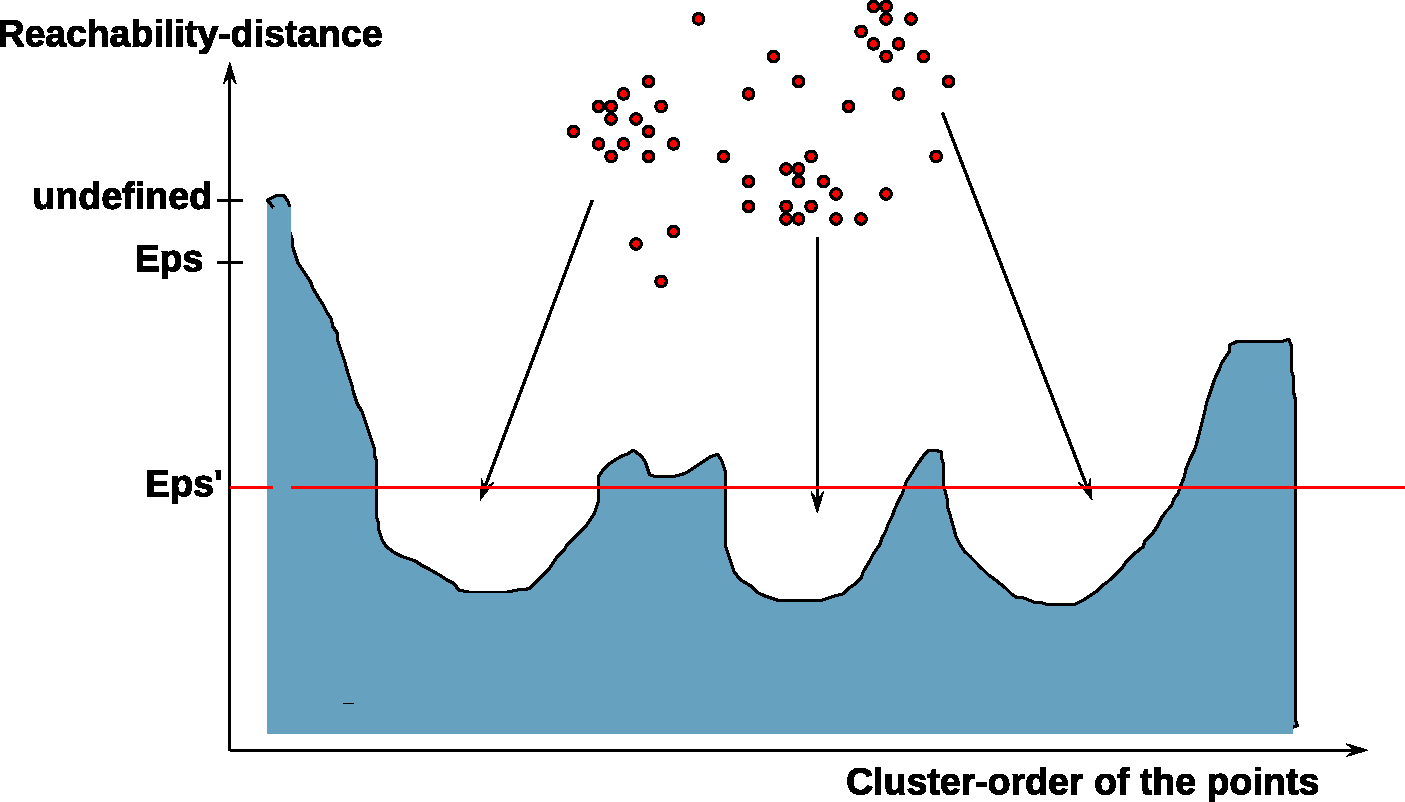
\includegraphics[width=10.5cm]{img/clusterdensity.pdf}
\end{frame}

\begin{frame}{DENCLUE: Using Statistical Density Functions}
	\begin{itemize}
		\item \textbf{DENsity-based CLUstEring}\footfullcite{hinneburg1998}
		\item \textbf{Using statistical density functions:}
		      \begin{itemize}
			      \item $f_{\text{Gaussian}}(x,y)=
				            \exp\left(\frac{d(x,y)^2}{2\sigma^2}\right)$, influence of $y$ on
			            $x$.
			      \item $f^D_{\text{Gaussian}}(x,x_i)= \sum_{i=1}^{N}
				            \exp\left(\frac{d(x,x_i)^2}{2\sigma^2}\right)$, total influence on
			            $x$.
			      \item $\nabla_{x_i} f^D_{\text{Gaussian}}(x,x_i) = \sum_{i=1}^{N}
				            (x_i-x) \cdot \exp\left(\frac{d(x,x_i)^2}{2\sigma^2}\right)$,
			            gradient of $x$ in direction $x_i$.
		      \end{itemize}
		\item \textbf{Major features:}
		      \begin{itemize}
			      \item Solid mathematical foundation.
			      \item Good for data sets with large amounts of noise.
			      \item Allows a compact mathematical description of arbitrarily
			            shaped \\
			            clusters in high-dimensional data sets.
			      \item Significantly faster than existing algorithms (e.g., DBSCAN).
			      \item But needs a large number of parameters.
		      \end{itemize}
	\end{itemize}
\end{frame}

\begin{frame}{DENCLUE: Technical Essence}
	\begin{itemize}
		\item \textbf{Density estimation:}
		      \begin{itemize}
			      \item Estimation of an unobservable underlying probability density
			            function based on a set of observed data.
			      \item Regarded as a sample.
		      \end{itemize}
		\item \textbf{Kernel density estimation:}
		      \begin{itemize}
			      \item Treat an observed object as an indicator of high-probability
			            density in the surrounding region.
			      \item Probability density at a point depends on the distances from
			            this point to the observed objects.
		      \end{itemize}
		\item \textbf{Density attractor:}
		      \begin{itemize}
			      \item Local maximum of the estimated density function.
			      \item Must be above threshold $\xi$.
		      \end{itemize}
	\end{itemize}
\end{frame}

\begin{frame}{DENCLUE: Technical Essence (II)}
	\begin{itemize}
		\item \textbf{Clusters:}
		      \begin{itemize}
			      \item Can be determined mathematically by identifying density
			            attractors.
			      \item That is, local maxima of the overall density function.
		      \end{itemize}
		\item \textbf{Center-defined clusters:}
		      \begin{itemize}
			      \item Assign to each density attractor the points density-attracted
			            to it.
		      \end{itemize}
		\item \textbf{Arbitrary shaped cluster:}
		      \begin{itemize}
			      \item Merge density attractors that are connected through paths of
			            high density ($>$ threshold).
		      \end{itemize}
	\end{itemize}
\end{frame}

\begin{frame}{Density Attractor}
	\centering
	\vspace{1cm}
	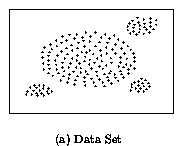
\includegraphics[width=4cm]{img/densityattractor.png}
	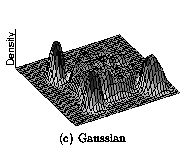
\includegraphics[width=4cm]{img/densityattractor1.png}
	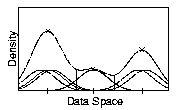
\includegraphics[width=4cm]{img/densityattractor2.png}
\end{frame}

\begin{frame}{Density Attractor}
	\centering
	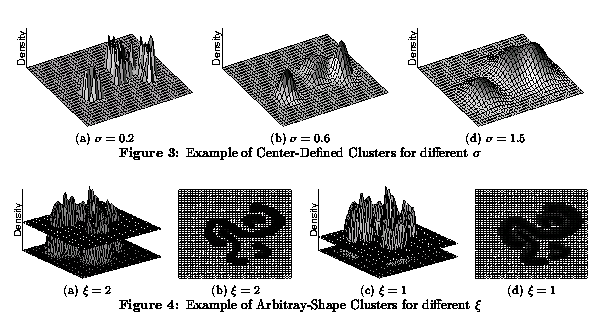
\includegraphics[width=11.5cm]{img/densities.png}
\end{frame}
